\documentclass[class=article, crop=false]{standalone}
\usepackage{tikz}
\usepackage{subcaption}
\usetikzlibrary{calc}

\begin{document}
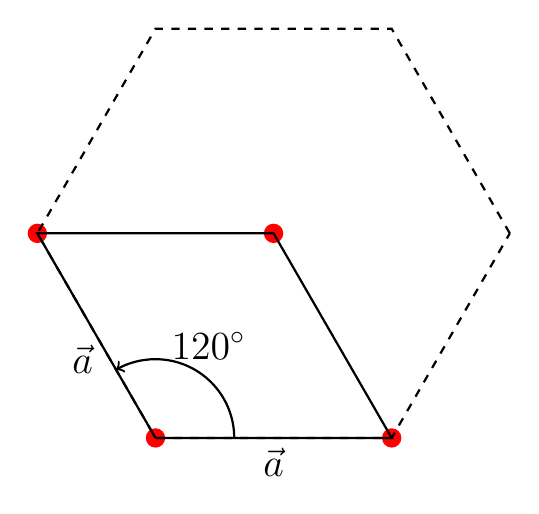
\begin{tikzpicture}
    \def\a{3}  % length of side a

    Calculate the coordinates of the points
    \coordinate (A) at (0:\a);
    \coordinate (B) at (60:\a);
    \coordinate (C) at (120:\a);
    \coordinate (D) at (180:\a);
    \coordinate (E) at (240:\a);
    \coordinate (F) at (300:\a);
    \coordinate (G) at (0,0);


    % Creates nodes at vertices
    \fill[red]  (D) circle(3.5pt) (E) circle(3.5pt) (F) circle(3.5pt) (G) circle(3.5pt);
    

    % Draw the hexagon boundary
    \draw[thick,dashed] (A) -- (B) -- (C) -- (D) -- (E) -- (F) -- (A);

    % Draw the cell
    \draw[thick] (E) -- (F) -- (G) -- (D) -- (E); 

    %Draw lattice parameters
    \node[anchor={60}] at ($(D)!0.5!(E)$) {\Large $\vec{a}$};
    \node[below] at ($(E)!0.5!(F)$) {\Large $\vec{a}$};

    % Optional: add angle markers
    \draw[thick, ->] (E) ++(1,0) arc[start angle=0, end angle=120, radius=1] node[midway,anchor={-120}] {\Large $120^\circ$};
    
\end{tikzpicture}
\end{document}